\section{Introduction}
In order to achieve the navigation services we have to find the position and velocity of satellite in its orbit.In order to find the position and velocity we have the source called RINEX file Which contains all the orbital parameters of the satellite in its orbit.In this document we  compute the position and velocity of GPS and NAVIC satellites.The RINEX files is different for both the satellites but the algorithm for finding the position and velocity is same.
\subsection{Determination of position}
RINEX files will be available in official websites for all the satellites.
The RINEX files contains all the information of the orbital parameters of the particular satellite.The Orbital elements of satellite from rinex file is given in below table.
\subsection{Orbital parameters in rinex file}
\begin{tabular}{ | m{10em} | m{10cm} | } 
  \hline
  $\sqrt{a}$   & Square rooot of semimajor axis \\
  \hline
  e & 
  Eccentricity \\  
  \hline
  $\Delta$n & Mean motion diffeerence from computed value  \\
  \hline
  $M_0$ & Mean anom
  maly at reference time \\
  \hline
  $\Omega_0$ & Longitude of ascending node
  n
  of orbit plane at weekly epoch  \\
  \hline
  $i_0$ & Inclination angle
  a
  at reference time   \\
  \hline
  w & Argum
  ment of perigee \\
  \hline
$\Omega_.$& Rate of right ascension  \\
  \hline
  IDOT & Rate off inclination angle  \\
  \hline
$t_{oe}$  & Ephemeeris reference time  \\
  \hline
  IODE  &  Issue of data, ephemeris \\
  \hline
  $C_{uc}$ & Amplitude of cosine harmonic
  h
  correction term to the
  argum
  ment of latitude   \\
  \hline
  $C_{us}$& Amplitude of sine harmonnic correction term to the argument
  of latitude \\
  \hline
  $C_{rc}$  &  Amplitude of cosine harrmonic correction term to the orbit
  radius \\
  \hline
  $C_{rs}$ & Amplitude of sine harm
  monic correction term to the orbit
  radius  \\
  \hline
  $C_{ic}$ & Amplitude of cosine harm
  monic correction term to the angle of
  i
  inclination \\
  \hline
  $C_{is}$ & Amplitude of sine harmoonic correction term to the angle of
  i
  inclination  \\
  \hline
\end{tabular}
\begin{figure}
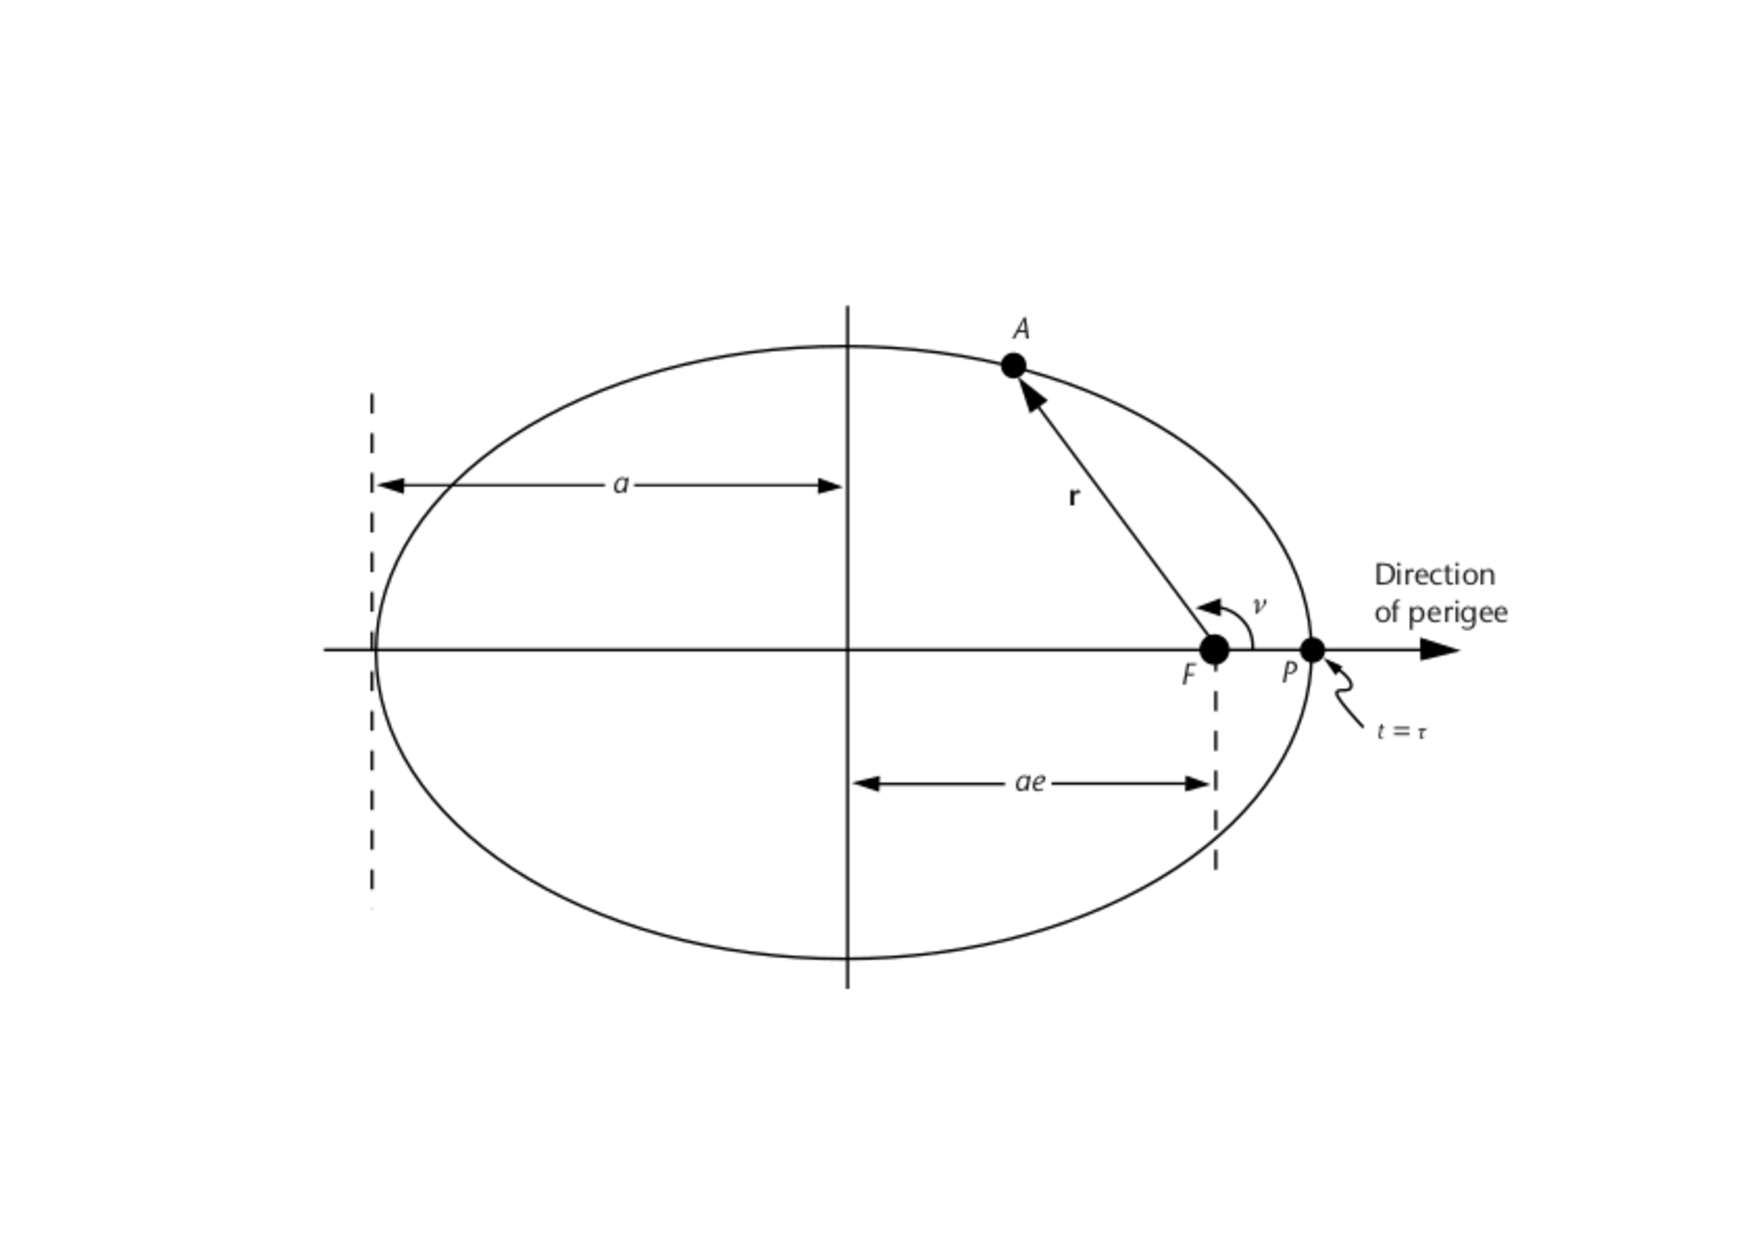
\includegraphics[scale=0.4]{figs/1.pdf}
\end{figure}
\vspace{30cm}
\\
In the above Figure 
\begin{enumerate}
\item The elliptical orbit has a focus at point
F, which corresponds to the center of the mass of the Earth.
\item The time t0 at which the satellite is at some
reference point A in its orbit is known as the epoch.
\item The point, P, where the satellite is closest to the center of the Earth
is known as perigee.
\item The time at which the satellite passes perigee,t, is another
Keplerian orbital parameter.
\end{enumerate}
\vspace{5mm}
The three Keplerian orbital elements
that define the shape of the elliptical orbit and time relative to perigee are as
follows:
\begin{enumerate}
  \item a = Semimajor axis of the ellipse
  \item e = eccentricity of the ellipse
  \item t = time of perigee passage
\end{enumerate}
In order to find the position of satellite let us understand the keplerian orbital elements.\\
\\
\textbf{True anamoly :} The angle in the orbital plane measured counterclockwise from
the direction of perigee to the satellite.\\ 
\\
\textbf{Eccentric anamoly :} Geometrically, the eccentric anomaly is constructed from the true anom-
aly first by circumscribing a circle around the elliptical orbit. Next, a perpendicular
is dropped from the point A on the orbit to the major axis of the orbit, and this per-
pendicular is extended upward until it intersects the circumscribed circle at point B. The angle measured at the center of the circle, O, counter-
clockwise from the direction of perigee to the line segment.
\begin{figure}
  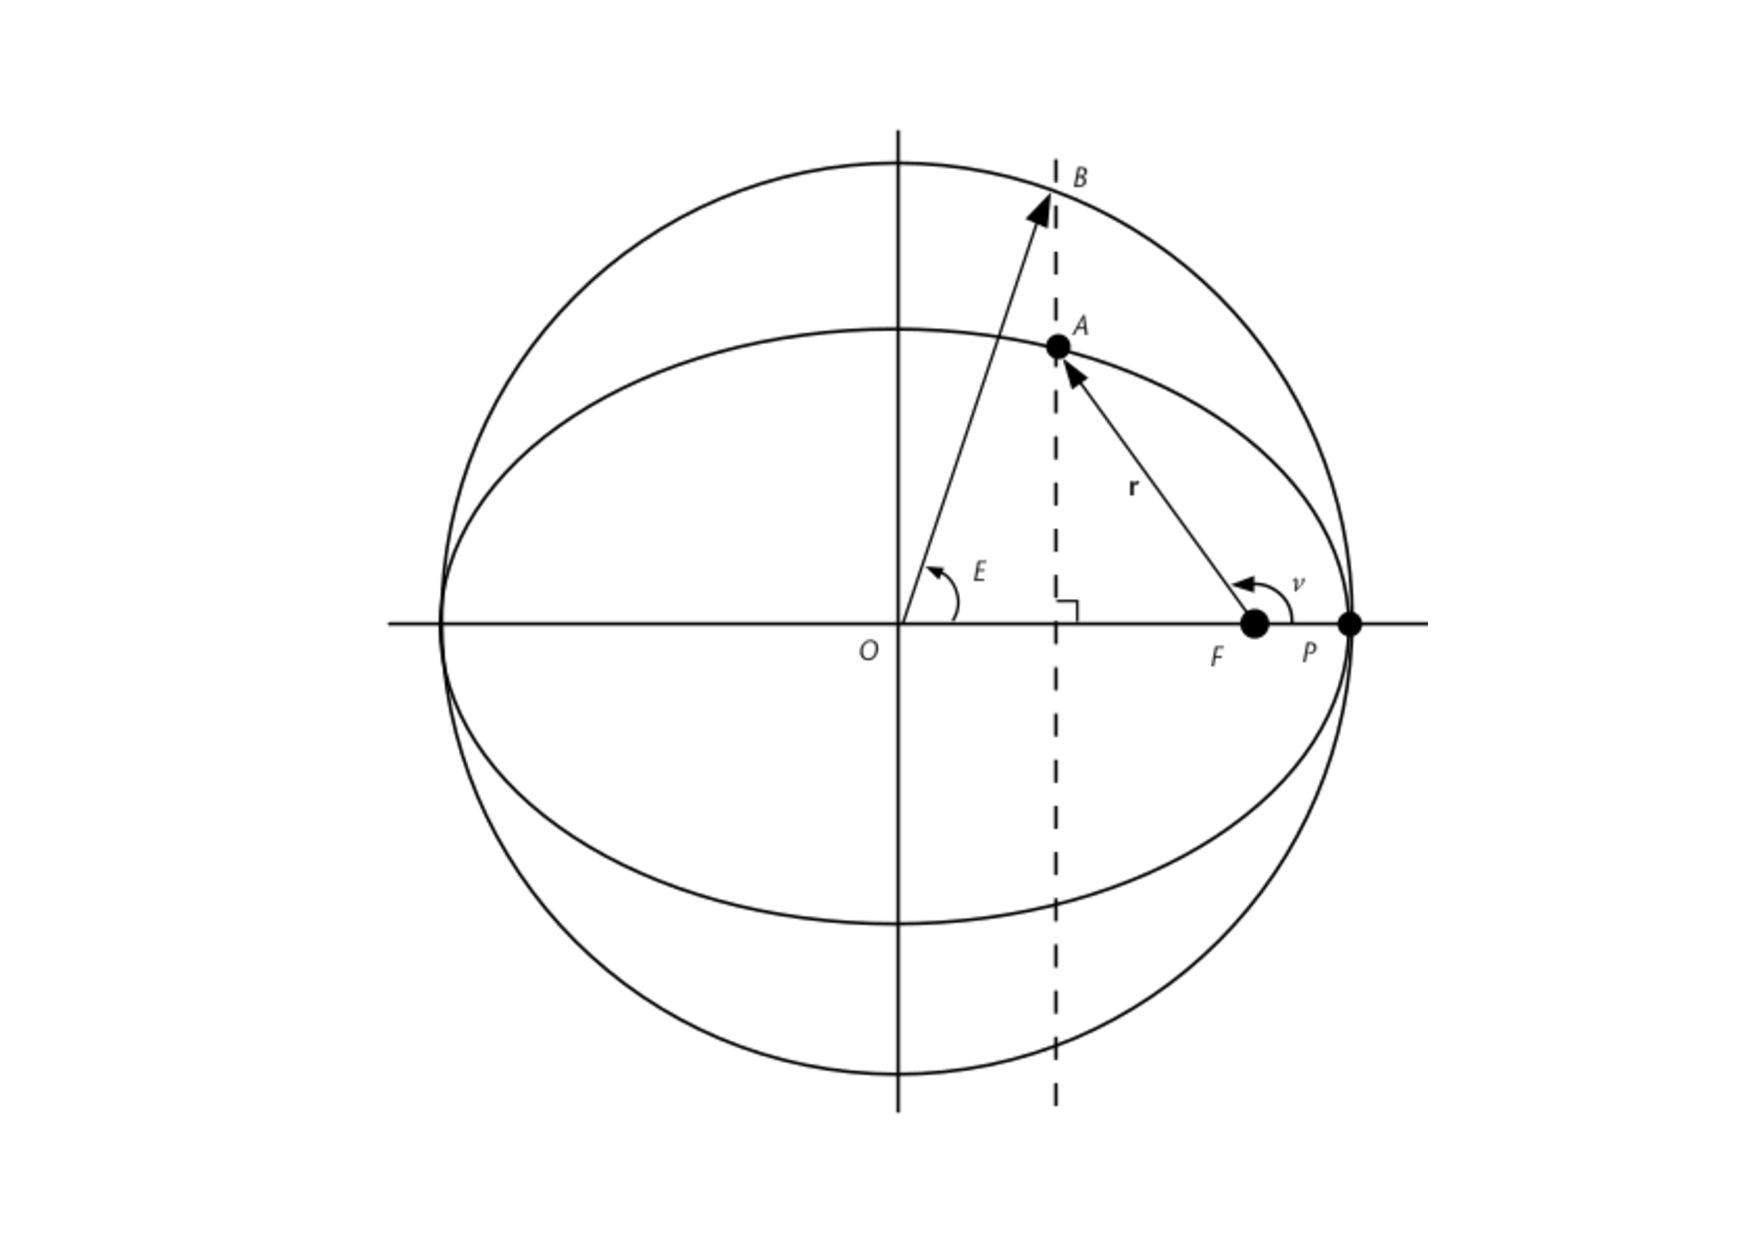
\includegraphics[scale=0.4]{figs/2.pdf}
  \end{figure}
 \begin{align}
E&=2\arctan (\sqrt{\frac{1+e}{1-e}}\tan(\frac{v}{2})  )
 \end{align}
 \\
 \textbf{Mean anamoly :} The importance of transforming from the true to the mean
 anomaly is that time varies linearly with the mean anomaly.\\
 \begin{align}
  M&=M_o+n*(t-t_o)
 \end{align}
 Where,\\
 $M_o$ is Mean anamoly at the time of epch.\\
 M is the mean anomaly at time t.\\
 \begin{align}
  n&=\sqrt{\frac{\mu }{a^3}} \\
  \mu&=398,600.5 * 10^8 m^3/s^2
 \end{align} 
 \\
 In the case of GPS or Navic, the Keplerian
parameters are defined in relation to the ECEF coordinate system .In this case, the xy-plane is always the Earth's equatorial plane.
The following three Keplerian orbital elements define the orientation of the orbit in the
ECEF coordinate system:\\
\\
\textbf{Inclination of orbit :} Inclination is the dihedral angle between the Earth’s equatorial plane and the
satellite’s orbital plane.\\
\\
\textbf{longitude of the ascending node :} The orbital element that defines the
angle between the +x-axis and the direction of the ascending node is called the right
ascension of the ascending node (RAAN). Because the +x-axis is fixed in the direc-
tion of the prime meridian (0° longitude) in the ECEF coordinate system, the right
ascension of the ascending node is actually the longitude of the ascending node,$\Omega$.\\
\\
\textbf{Arguement of perigee :} Measures the angle
from the ascending node to the direction of perigee in the orbit. \\
\\
Notice that $\Omega$ is measured in the equatorial plane, whereas $\omega$ is measured in the orbital plane.
The following formulas are used for computing the position,velocity of the satellite in the elliptical orbit.Where the inputs are taken from the rinex file.
\begin{align}
  \Omega^. &= 7.2921151467*10^{-5} rad/sec \\
  a&=\sqrt{a^2} \\
  t_k&=t-t_oe \\
  n&=n_o+\Delta n \\
  M_k&=M_o+nt_k \\
  E_k&=M_k+e\sin(E_k) \\
  \sin(v_k) &=\frac{1 - e^2sin E_k}{1 - ecos E_k}\\
\cos(v_k)&=\frac{\cos(E_K)-e}{1-ecos(E_k)} \\
\phi_k&=v_k+w \\
\delta \phi_k &= C_{us}\sin(2 \phi_k ) + C_{uc}\cos(2 \phi_kk ) \\
\delta r_k &= C_{rs}\sin(2 \phi_k ) + C_{rc}\cos(2 \phi_k ) \\
\delta i_k &= C_{is}\sin(2 \phi_k ) + C_{ic}\cos(2 \phi_k ) \\
u_k&= \phi_k + \delta \phi_k \\
r_k &= a(1 - e\cos E_k ) + \delta r_k \\
i_k &= i_0 + \frac{di}{dt}t_k + \delta i_k \\
\Omega_k &= \Omega_0 + \Omega^. - \Omega_e^. (t_k ) - \Omega_e^. t_{oe} \\
x_p &= r_k \cos(u_k) \\
y_p &= r_k \sin(u_k) \\
x_s &= x_p \cos \Omega_k - y_p \cos i_k \sin \Omega_k \\
y_s &= x_p \sin \Omega_k - y_p \cos i_k \cos \Omega_k \\
z_s &= y_p \sin i_k
\end{align}
\\
By computing the above formulas [$x_s,y_s,z_s$] are the position of satellite in ECEF cooedinate frame.\\
The velocity of the satellite is obtained by differentiating the above position equations with respect to time.The final equation is as follows: 
\\
\\
$x_v = -x_p \Omega_k^. \sin \Omega_k + x_p^. \cos \Omega_k - y_p^. \sin \Omega_k \cos i_k$ \\
$-y_p(\Omega_k^.\cos \Omega_k \cos i_k - \frac{dik}{dt} \sin \Omega_k \sin i_k )$ \\
\\
$y_v = -x_p \Omega_k^. \cos \Omega_k + x_p^. \sin \Omega_k - y_p^. \cos \Omega_k \cos i_k$ \\
$-y_p(\Omega_k^.\sin \Omega_k \cos i_k - \frac{dik}{dt} \cos \Omega_k \sin i_k )$ \\
\\
$z_v = y_p\frac{di_k}{dt}\cos i_k + y_p^.\sin i_k$
\\
\\
By computing the above formulas $[x_v,y_v,z_v]$ is the velocity vector of satellite in ECEF coordinate frame. 
\\
\\
\textbf{Computations of error corrections :} 
\begin{enumerate}
  \item \textbf{Clock Correction :} \\
One of the largest sources of error in calculating range is
satellite clock error. To get the accuracy of the receiver
position signal transmission and reception time must be
precisely known. Because of the travel time of light, one
nanosecond of inaccuracy in the clock causes 30 centimeter
error in position. Satellite clock correction coefficients - clock
bias, clock drift, and clock drift rate are obtained from the
RINEX Navigation file. Calculation of the satellite clock error
is given by 
\begin{align}
\Delta t_{clk}&=a_{f0} + a_{f1}(t-t_{oc}) + a_{f2}(t-t_{oc})^2
\end{align}
where ,\\
$\Delta t_{clk}$ is clock offset in seconds.\\
t is IRNSS system time at transmission in seconds.\\
$t_{oc}$ is clock data reference time. \\
$a_{f0}$ is clock bias. \\
$a_{f1}$ is clock drift.\\
$a_{f2}$ is clock drift rate.
\item \textbf{Relativistic Correction :} \\
Because of the high speed of satellites and
weaker gravity, clocks on the satellites run a little faster than the clock on the Earth. Error found because the relativity is in
nanoseconds. The computation of relativistic clock error is given
by
\begin{align}
\delta _{rel}&=Fe\sqrt{a}\sin (E)
\end{align}
where ,\\
a is semimajor axis of the ellipse. \\
e is eccentricity of the ellipse. \\
F is -4.442807633 * $10^{-10}$ \\
E is Eccentric anamoly.
$\delta _{rel}$ is relativistic clock correction \\
\end{enumerate}
\section{Computing the position and velocity of the  GPS satellite using python}
\textbf{Installations :}
\begin{enumerate}
\item pip3 install pymap3d
\item pip3 install georinex
\item pip3 install itertools
\item pip3 install argparse
\end{enumerate}
\textbf{Algorithm for finding the position and velocity of satellite From Rinex file :}
\begin{enumerate}
  \item Get the rinex file for GPS  satellite from the official website.
  \item The Rinex file contains the observational file and navigation file.
  \item Convert the Rinex file to CSV file using the python \\
  The below python function will convert the GPS RINEX file to CSV file.
  \begin{lstlisting}
    ./rinex_to_csv/funcs.py
  \end{lstlisting}
  \item Remove the empty rows in csv file.The python function for removing empty rows is 
  \begin{lstlisting}
    ./rinex_to_csv/funcs.py
  \end{lstlisting}
  \item Convert the csv file to list in python so that each row is corresponds to the parameters of the satellite. Function for converting the csv file to list is given as :
  \begin{lstlisting}
    ./rinexread/funcs.py
  \end{lstlisting} 
  \item Process the above list with the formulas mentioned in chaprter 2 \\
  The python function for finding the position of satellite is given as :
  \begin{lstlisting}
    ./position/funcs.py
  \end{lstlisting}
  \item The velocity of the satellte is computed by the function 
  \begin{lstlisting}
    ./velocity/funcs.py
  \end{lstlisting}
  \item The distance between the satellite and receiver is obtained by the python package called \textbf{pymap3d},using this package convert ECEF to spherical coordinate frame.So that we obtain the distance between satellite and receiver.
  \item These position and velocity of the satellite is used for computing the doppler shift.
\end{enumerate}
\vspace{5mm}
The above alogorith will work for both GPS and Navic sarellite.If there is a problem in converting Navic RINEX file to csv file then follow the instructions below:
\begin{enumerate}
\item go to the mentioned folder in your laptop.
\begin{lstlisting}
  ./home/mannava/.local/lib/python3.10/site-packages/georinex/nav3.py
\end{lstlisting}
\item Go to the line 220 in nav3.py file and modify the below changes.
\begin{lstlisting}
  elif numval == 29:  # only one trailing spare fields
            cf = cf[:-2]
        elif numval == 28:  # only one trailing spare fields
            cf = cf[:-3]
        elif numval == 27:  # only one trailing spare fields
            cf = cf[:-4]
        elif numval == 26:  # only one trailing spare fields
            cf = cf[:-5]
\end{lstlisting}
\end{enumerate}
